\def\mySecNum{13.3}
\mySection{\mySecNum~Delta-Hedging}
%-------------- start slide -------------------------------%{{{ 1 Table 13.2
\begin{frame}[fragile,t]
 \begin{center}
   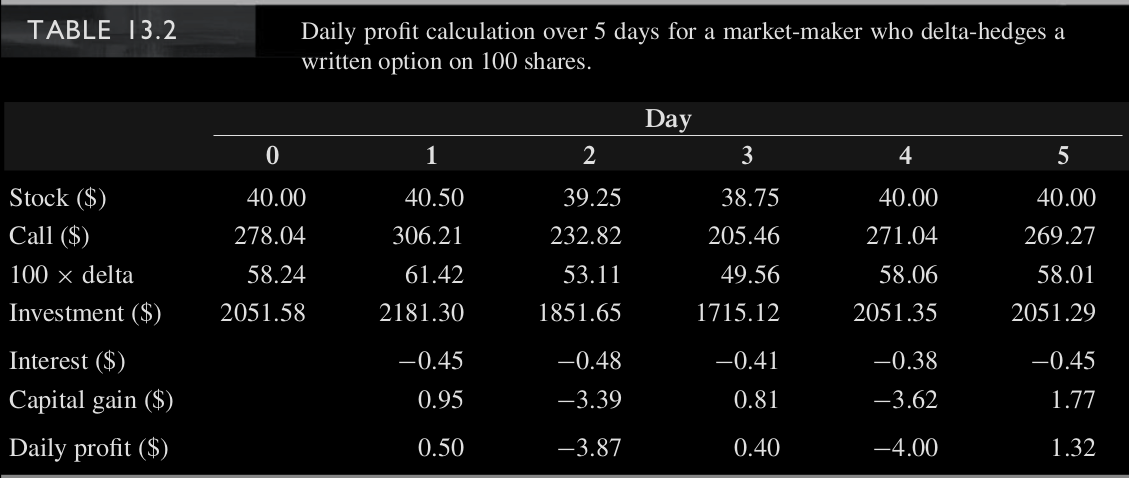
\includegraphics[scale=0.25]{figs/Table_13-2.png}
 \end{center}
 \begin{myexample}
   Given the first line of the above table, filling all the rest entries.
 \end{myexample}
 \begin{mysol}
   Check \textcolor{gray}{codes/Section\_13-2.nb}\myEnd
 \end{mysol}
\end{frame}
%-------------- end slide -------------------------------%}}}
%-------------- start slide -------------------------------%{{{ 1 Table 13.3
\begin{frame}[fragile,t]
  \frametitle{Self-financing portfolio: stock moves one $\sigma$}
 \begin{center}
   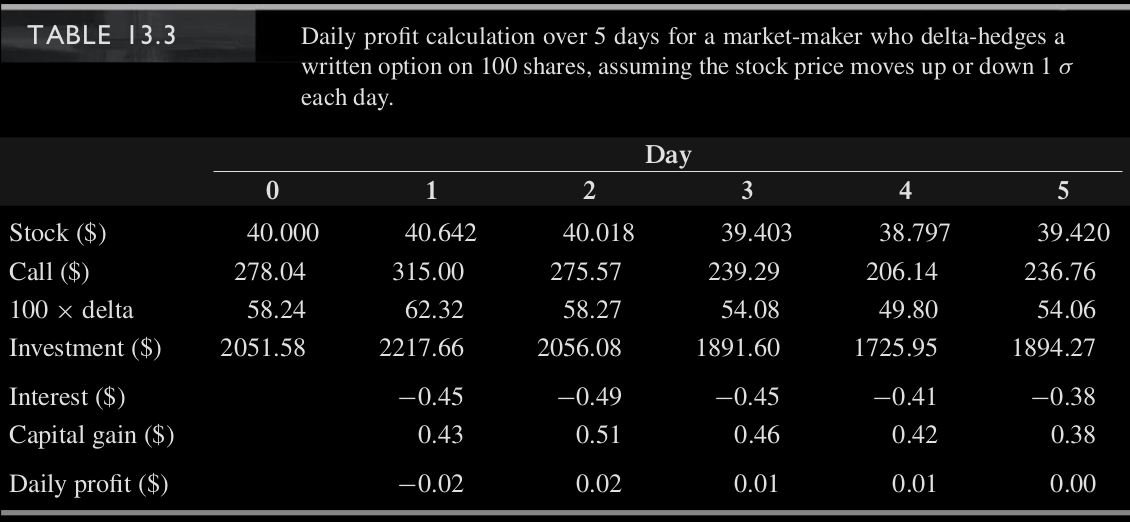
\includegraphics[scale=0.25]{figs/Table_13-3.png}
 \end{center}
 \begin{myexample}
   Given the first line of the above table, filling all the rest entries.
 \end{myexample}
 \begin{mysol}
   Check \textcolor{gray}{codes/Section\_13-2.nb}\myEnd
 \end{mysol}
\end{frame}
%-------------- end slide -------------------------------%}}}
